\documentclass{beamer}
\usepackage{lmodern}
\usepackage[utf8]{inputenc}

\usepackage{enumerate}
\usepackage{multimedia}

\usetheme{polimix}
\usepackage{natbib}
 
\title[Safe Policy Optimization]{Safe Policy Optimization}
\subtitle{{\small Ph.D. Course in Information Technology, XXXIII cycle} \\Second Annual Report}

\author[M. Papini]{Matteo Papini}
\supervisor{\small Supervisor}{\small Marcello Restelli}
\date[30/9/2019]{\small 30 Settembre 2019}

\begin{document}

%%%%%%%%%%%%%%%%%%%%%%%%%%%%%%%%%%%%%%%%%%%%%%%%%%%%%%%%%%%%%%%%%%%%%%%%%%%%%%%%%%%%%%%%%%%%%%%%%%%%%%%%%%%%%%%%%%%%
\begin{frame}
\titlepage
\end{frame}

\addtocounter{framenumber}{-1}

%%%%%%%%%%%%%%%%%%%%%%%%%%%%%%%%%%%%%%%%%%%%%%%%%%%%%%%%%%%%%%%%%%%%%%%%%%%%%%%%%%%%%%%%%%%%%%%%%%%%%%%%%%%%%%%%%%%%
\begin{frame}
\frametitle{Motivation}
Apply \textbf{Reinforcement Learning} to \textbf{real-world} control problems
\vfill
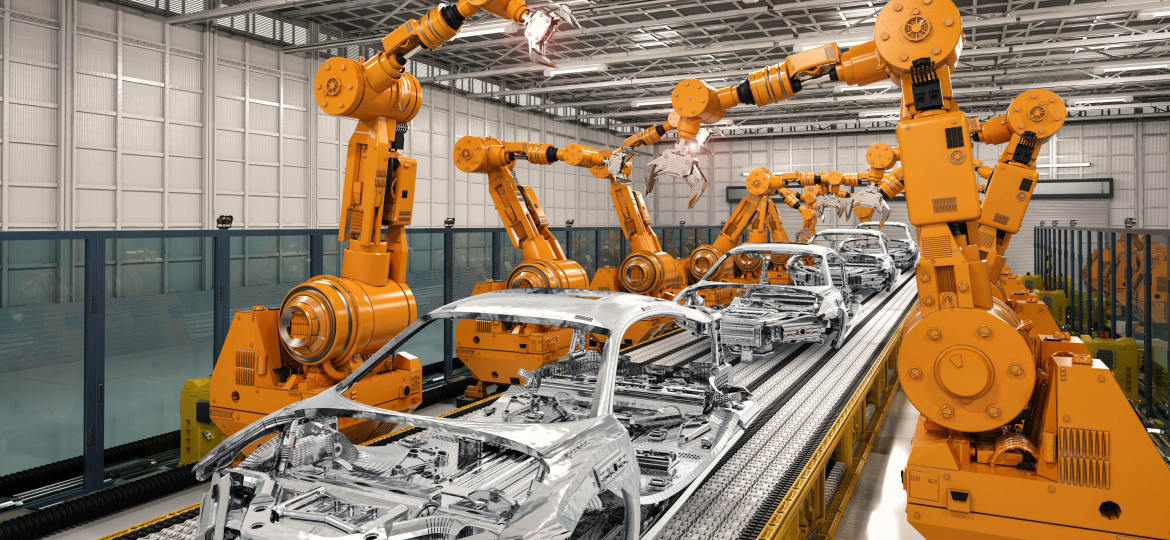
\includegraphics[width=\textwidth]{pics/factory.jpg}
\end{frame}

\addtocounter{framenumber}{-1}
\begin{frame}[plain]
\tableofcontents
\end{frame}

%%%%%%%%%%%%%%%%%%%%%%%%%%%%%%%%%%%%%%%%%%%%%%%%%%%%%%%%%%%%%%%%%%%%%%%%%%%%%%%%%%%%%%%%%%%%%%%%%%%%%%%%%%%%%%%%%%%
\section{Policy Optimization in the Real World}
%\addtocounter{framenumber}{-1}
%\frame{\tableofcontents[currentsection]}

\begin{frame}
\frametitle{Reinforcement Learning}
\centering
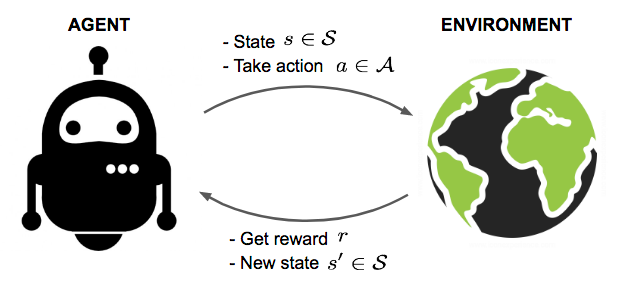
\includegraphics[width=.75\textwidth]{pics/rl2.png}\\
\vspace{.5cm}
{\bf Policy:} agent's behavior ($s\mapsto a$) \\
{\bf Performance $\rho$:} \emph{expected} total reward \\
{\bf Goal:} find policy maximizing performance
\vspace{.25cm}
\begin{itemize}
	\item Model-free
	\item Online
	\item Iterative
\end{itemize}
\end{frame}

\begin{frame}
\frametitle{Continuous Reinforcement Learning}
Interesting real-world control problems are \textbf{continuous}
\begin{center}
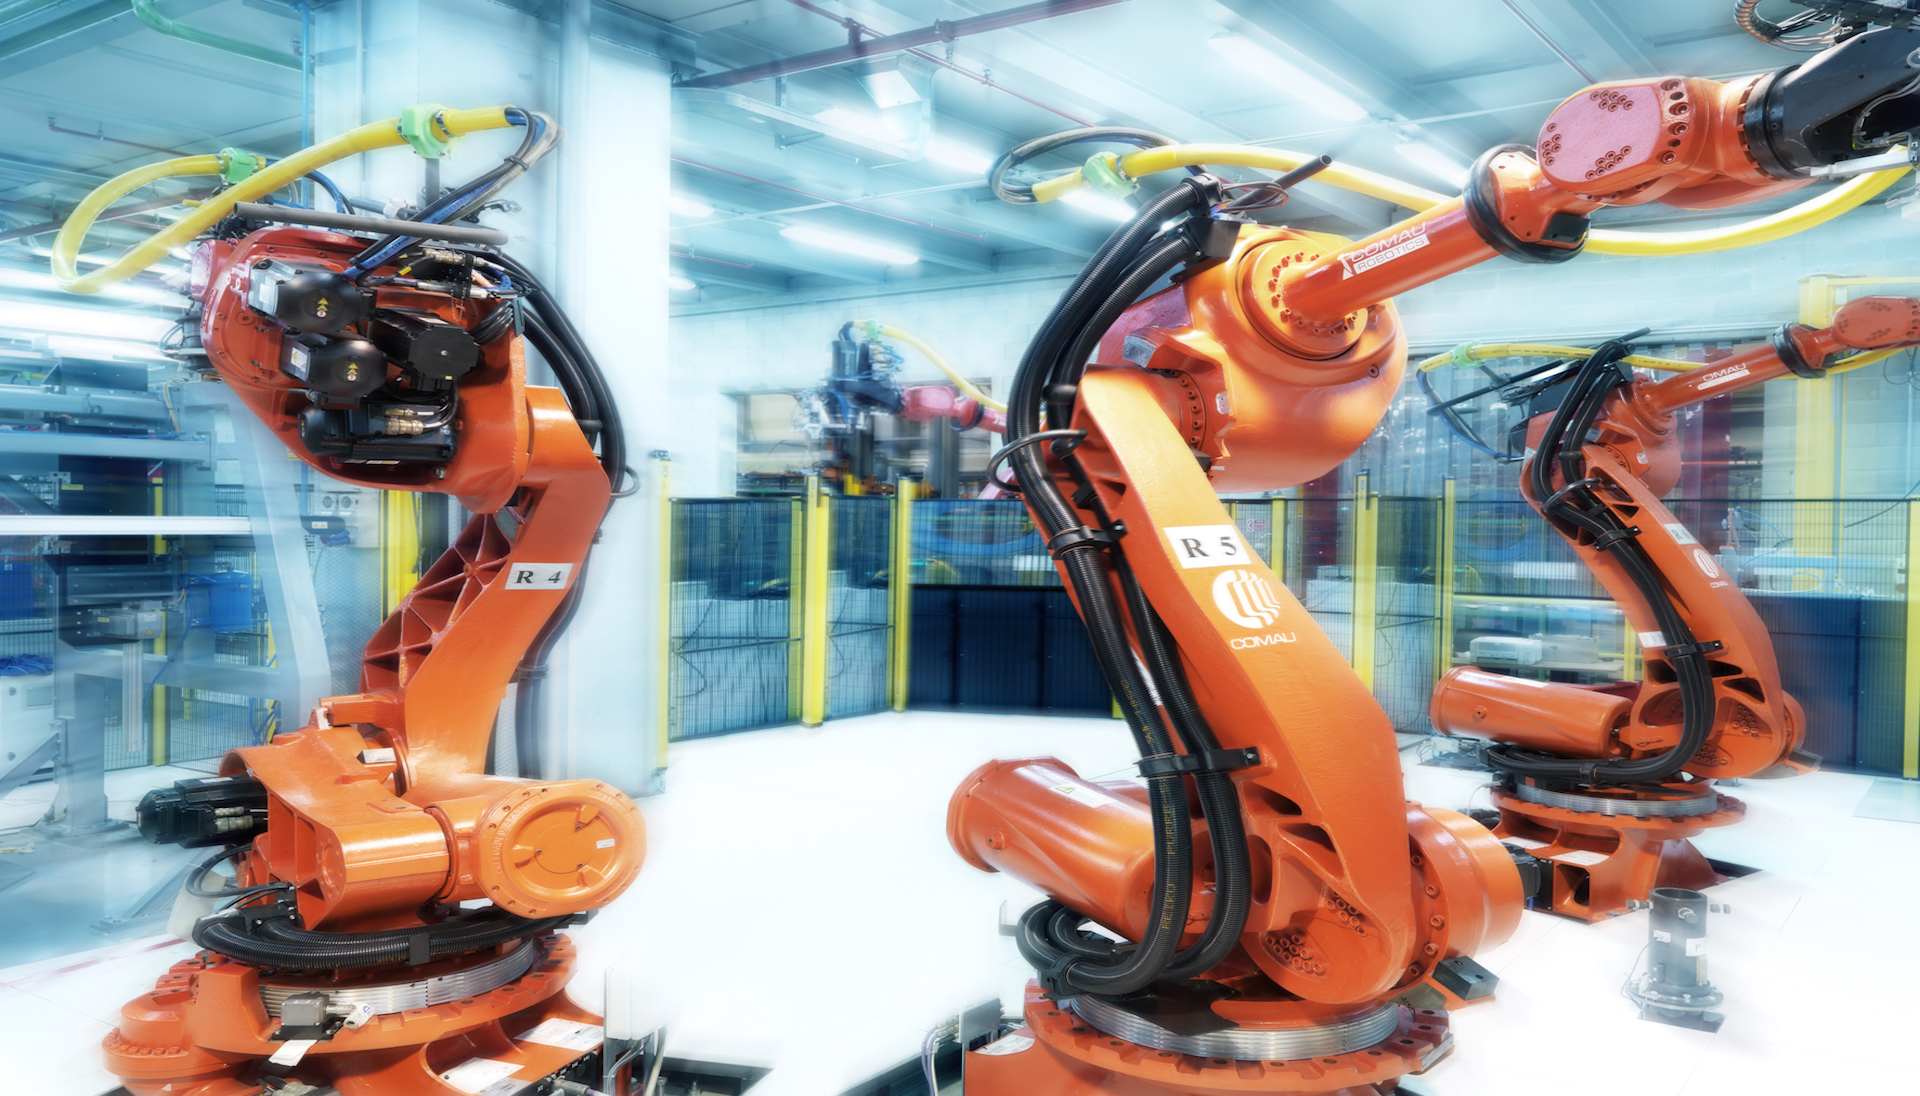
\includegraphics[width=.5\textwidth]{pics/robots.jpg}
\end{center}
\textbf{Policy Optimization:}
\begin{itemize}
	\item Scales well with state-action dimensionality
	\item Convergence guarantees
	\item Robustness to noise
\end{itemize}
\end{frame}

\begin{frame}
\frametitle{Policy Optimization}
\begin{itemize}
	\item Fix a class of controllers with tunable parameters $\boldsymbol{x}\in\mathcal{X}$
	\item Find policy parameters maximizing performance:
	\[	\LARGE
		\max\limits_{\boldsymbol{x}\in\mathcal{X}} \rho(\boldsymbol{x})
	\]
	\vfill
	\item \textbf{Policy Gradient:} solve it with \emph{Stochastic Gradient Descent}
	\vfill
	\begin{columns}
		\begin{column}{.5\textwidth}
			\centering
			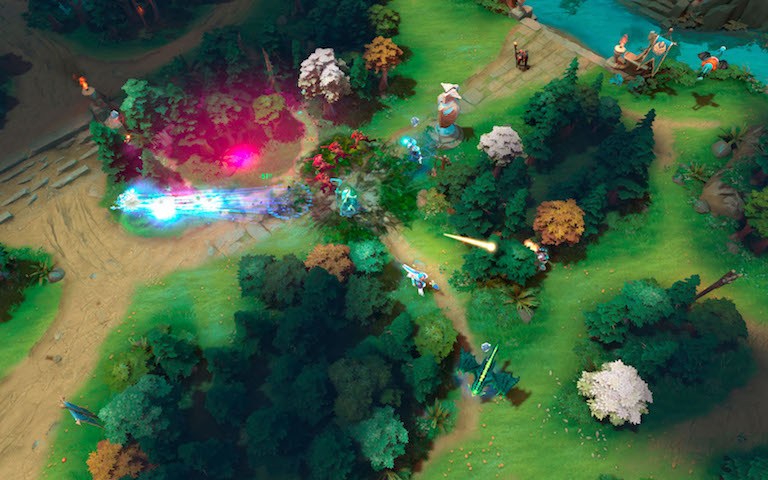
\includegraphics[width=.8\textwidth]{pics/dota.jpg}
			\\
			\emph{\cite{OpenAI_dota}}
		\end{column}
		\begin{column}{.5\textwidth}
			\centering
			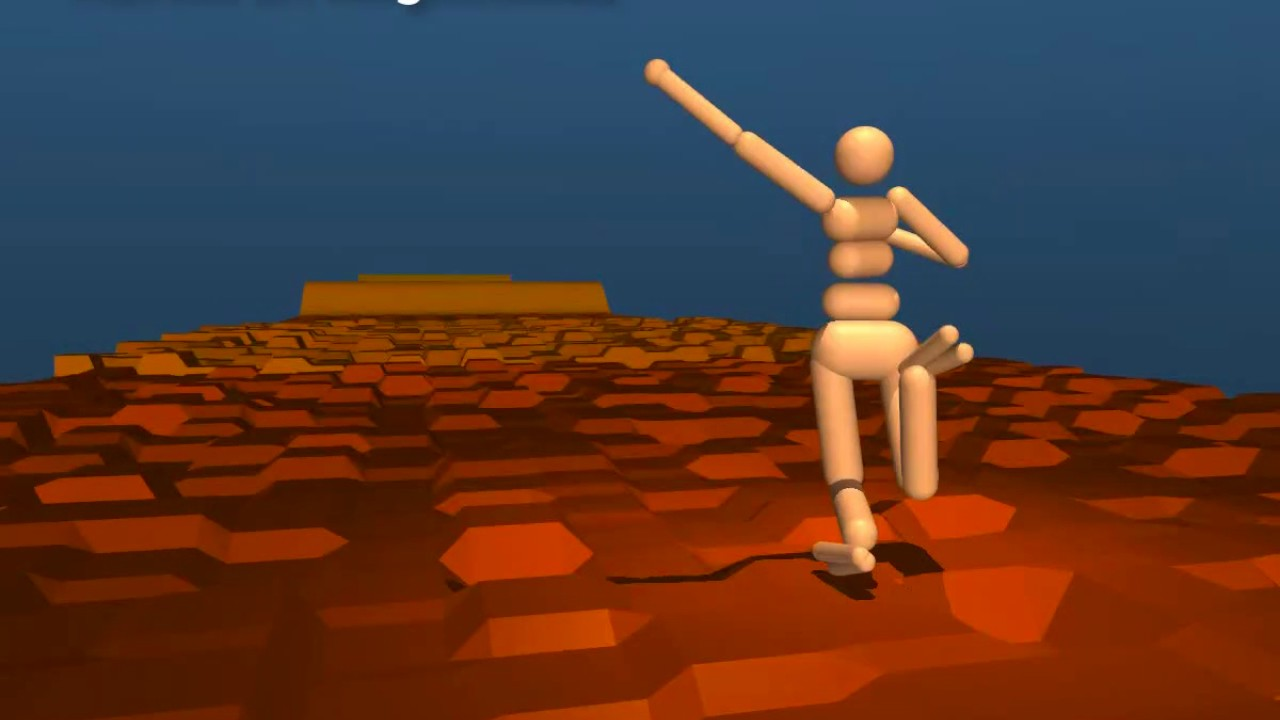
\includegraphics[width=.8\textwidth]{pics/parkour.jpg}
			\\ 
			\emph{\cite{heess2017emergence}}
		\end{column}
	\end{columns}
\end{itemize}
\end{frame}

\begin{frame}
\frametitle{Real-World Requirements}
\begin{columns}
	\begin{column}[t]{.5\textwidth}
		{\bf Boss:}\\
		\phantom{"I will improve your controller with RL!"}
		\vspace{1cm}
		\begin{itemize}
			\setlength{\itemsep}{10pt}
			\item How long will it take?
			\item Will it \emph{actually} improve?
			\item Will it behave safely?
			\item How much better will it become?
		\end{itemize}
	\end{column}
	\begin{column}[t]{.5\textwidth}
	{\bf ML Engineer:}\\ 
	"I will improve your controller with RL!"
	\vspace{1cm}
	\begin{itemize}
		\setlength{\itemsep}{10pt}
		\item[] Unknown \hfill \emph{sample complexity}
		\item[] Eventually \hfill \emph{safety}
		\item[] Eventually \hfill \emph{safety}
		\item[] Unknown \hfill \emph{quality of solutions}
	\end{itemize}
	\end{column}
\end{columns}
\end{frame}

%\begin{frame}
%\frametitle{Sample Complexity (First Year)}
%\textbf{Matteo Papini}, Damiano Binaghi, Giuseppe Canonaco, Matteo Pirotta, Marcello Restelli:
%\emph{Stochastic Variance-Reduced Policy Gradient}. \textbf{ICML 2018}: 4023-4032
%\vfill
%Alberto Maria Metelli, \textbf{Matteo Papini}, Francesco Faccio, Marcello Restelli:
%\emph{Policy Optimization via Importance Sampling}. \textbf{NeurIPS 2018}: 5447-5459
%\end{frame}

%%%%%%%%%%%%%%%%%%%%%%%%%%%%%%%%%%%%%%%%%%%%%%%%%%%%%%%%%%%%%%%%%%%%%%%%%%%%%%%%%%%%%%%%%%%%%%%%%%%%%%%%%%%%%%%%%%%
\section{Monotonic Performance Improvement}
\addtocounter{framenumber}{-1}
\frame{\tableofcontents[currentsection]}
\begin{frame}
\frametitle{Safety in Reinforcement Learning}
\begin{itemize}
	\setlength{\itemsep}{10pt}
	\item Many notions of safety ~\citep{amodei2016concrete,garcia2015comprehensive}
	\item Assume performance $\rho$ already encodes \emph{safety constraints}
	\item The optimal policy will be safe
	\item \textbf{The learning process itself may not be!}
\end{itemize}
\end{frame}

\begin{frame}
\frametitle{Monotonic Performance Improvement}
\begin{itemize}
	\item A concrete problem in Reinforcement Learning
\end{itemize}
\vfill
\centering
\includegraphics[width=.75\textwidth]{example-image-a}
\end{frame}

\begin{frame}
\frametitle{Smoothing Policies and Safe Policy Gradients}
\end{frame}

%%%%%%%%%%%%%%%%%%%%%%%%%%%%%%%%%%%%%%%%%%%%%%%%%%%%%%%%%%%%%%%%%%%%%%%%%%%%%%%%%%%%%%%%%%%%%%%%%%%%%%%%%%%%%%%%%%%
\section{Safe Exploration}
\addtocounter{framenumber}{-1}
\frame{\tableofcontents[currentsection]}

\begin{frame}
\frametitle{Safe Exploration}
\end{frame}

%\begin{frame}
%\frametitle{Safely Exploring Policy Gradients (?)}
%\end{frame}

\begin{frame}
\frametitle{OPTIMIST}
\end{frame}

\begin{frame}
\frametitle{(Truly) Deterministic Policy Gradient}
\end{frame}

%%%%%%%%%%%%%%%%%%%%%%%%%%%%%%%%%%%%%%%%%%%%%%%%%%%%%%%%%%%%%%%%%%%%%%%%%%%%%%%%%%%%%%%%%%%%%%%%%%%%%%%%%%%%%%%%%%%
\section{Quality of Solutions}
\addtocounter{framenumber}{-1}
\frame{\tableofcontents[currentsection]}

\begin{frame}
\frametitle{Non-Convexity}
\end{frame}

\begin{frame}
\frametitle{Global Optimality Guarantees}
\end{frame}

%%%%%%%%%%%%%%%%%%%%%%%%%%%%%%%%%%%%%%%%%%%%%%%%%%%%%%%%%%%%%%%%%%%%%%%%%%%%%%%%%%%%%%%%%%%%%%%%%%%%%%%%%%%%%%%%%%%

\begin{frame}
\frametitle{Wrapping Up}
\end{frame}

\begin{frame}
\frametitle{Publications}
\end{frame}

\begin{frame}
\frametitle{Courses and Schools}
\end{frame}

\begin{frame}
\frametitle{Teaching}
\end{frame}

\begin{frame}
\frametitle{Other Activities}
\end{frame}



\begin{frame}[plain]
\centering
{\color{poliblue3} \bf
\vspace{1cm}
{\huge Thank you for your attention!} \\
\vspace{2cm}
{\LARGE Questions?}
}
\end{frame}


\begin{frame}[allowframebreaks]
\frametitle{Bibliography}
\bibliographystyle{plainnat}
\bibliography{slides}
\end{frame}

%%%%%%%%%%%%%%%%%%%%%%%%%%%%%%%%%%%%%%%%%%%%%%%%%%%%%%%%%%%%%%%%%%%%%%%%%%%%%%%%%%%%%%%%%%%%%%%%%%%%%%%%%%%%%%%%%%%


\end{document} 
